\chapter{测试与评估}

\section{Benchmark测试}
下面我们将实现的MMT内存完整性保护原型,在SPECCPU和STREAM的测试集上进行测试。SPECCPU是一个标准的cpu,内存和io的综合测试,它选取了多个一个典型的应用场景,能够较好的反应机器的综合性能。STREAM是一个测试内存性能的测试集,有较大的内存压力,能够评估内存在极限情况的下的性能。
我们对比了不做任何完整性保护,使用SIT对内存进行完整性保护,使用vault对内存进行完整保护和使用MMT对内存进行完整性保护,在不同的测试集下的性能,同时页分析了页交换和Mount操作占总运行时间的比例,下面我们将具体的介绍每一个测试的结果。

\begin{figure}[!htp]
    \centering
    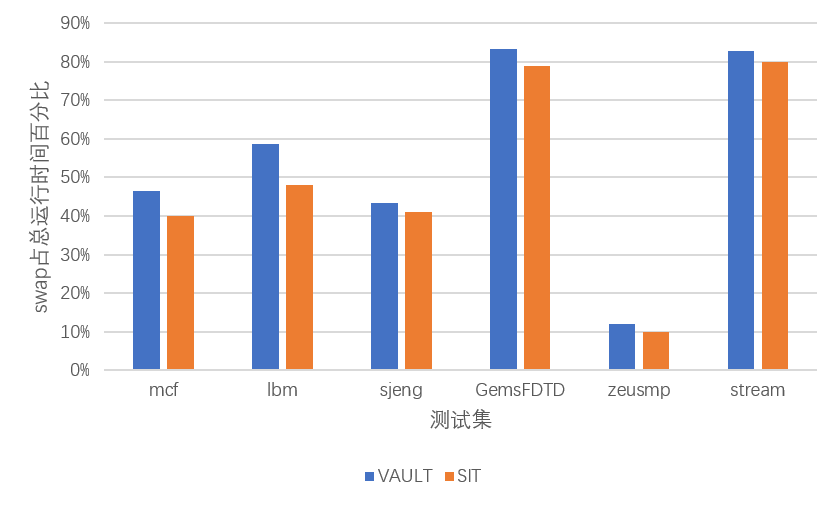
\includegraphics{eval-swap.png}
    \caption{\textbf{SPECCPU, STREAM测试集在不同完整性保护方案下swap所占比列}。}
   \label{fig:eval-swap}
\end{figure}
如图 ~\ref{fig:eval-swap}所示,我们分别测试了SIT,VAULT等先进的完整性保护方案,在超过soc上保护内存限制时候产生swap的开销占总运行时间的比例。为了能够理论上支持无限制的内存完整性保护方案,在SIT以及VAULT等方案中一旦使用的内存超过了soc可以保护的范围。CPU会选择恰当
页将其中改的数据进行加密,然后swap到非安全的内存中。为了保证从非安全内存中swap回到安全内存中,数据没有被修改。CPU在swap的时候会生成一个evict metatdate结构。该结构中记录了swap出去页的哈希值,以及属于哪一个enclave等相关的元数据,该结构被存储在安全内存中。注意当安全内存
十分紧张的时候,该数据结构也可能被swap到非安全内存中,同样我们会为存放evict metadata的页生成一个evict metadata,类似于树的形式,只需要保存根上的evict metadata既可以保证所有swap出去页的完整性。虽然SIT,vault能够理论上支持更多的内存,但是当SoC上保护得内存耗尽的时候
swap会带来很严重的性能开销,测试发现,一次swap将会带来高达40k的开销,我们在SPECCPU和STREAM测试集上进行了测试(这里我们挑选了SPECCPU中运行时内存超过128M的测试用例),我们发现swap占据了总运行时间的10\%-80\%,其中5/6的测试结果显示swap占据了总运行时间的40\%以上,其中GemsFDTD和STREAM测试swap的开销格外严重,占据了总运行时间的80\%以上,
另外杜比SIT和VAULT,在VAULT中swap的开销会更加的严重,这不是应为VAULT的设计的缺陷,还是因为VAULT运行时候的气态开销更小,导致了swap所占的时间更加明显。通过上面的数据显示,一旦使用的内存超过了SoC上保护的限制,swap将造成验证的性能降级,所以优化swap的开销非常的重要。

\begin{figure}[!htp]
    \centering
    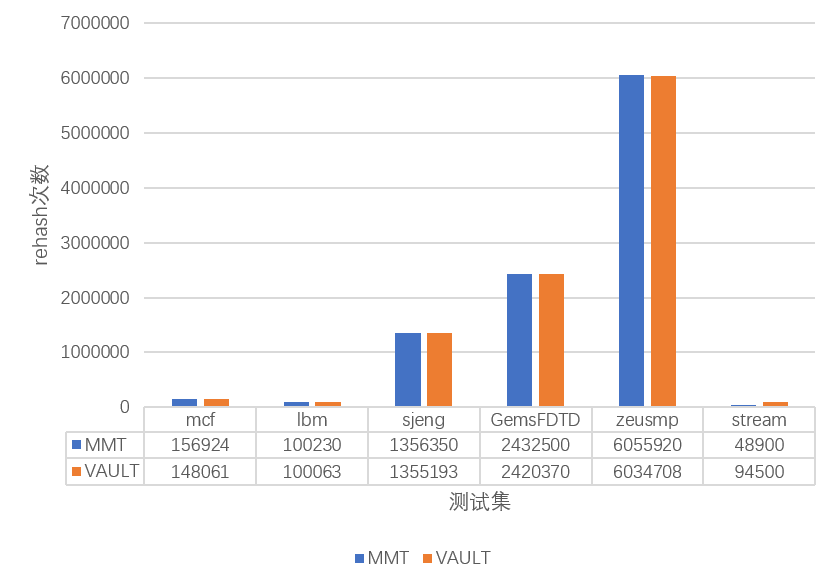
\includegraphics{eval-rehash.png}
    \caption{\textbf{SPECCPU, STREAM测试集在不同完整性保护方案下rehash的次数}。}
   \label{fig:eval-rehash}
\end{figure}
如图 ~\ref{fig:eval-rehash}所示,我们测试了VAULT和MMT中rehash的次数。为了能够增加完整性保护树中节点的扇出,VAULT和MMT都采用了分级counter的设计思路。因为分级counter会带来rehash的额外开销,来缓解replay等攻击。在MMT的设计中我们采用了三级counter的设计,三级counter的设计充分考虑了
完整性保护树中的冷热counter不均衡,在较高的树节点中往往只存在一个活跃的counter,而其他的counter可能处于不活跃的状态,所以我们可以减少冷counter比特数,增加热counter的比特数,从而兼顾安全性于节点的扇出。在这里我们同先进的VAULT完整性保护方案进行了比较。其中VAULT的稳定扇出为24,而MMT中
节点的扇出为32。在更大的扇出情况下,MMT并没造成更多的rehash的次数,说明在真实的workload下,完整性保护树中的冷热counter分布不均衡,而extra counter的设计能够很好的考虑到这种情况,从而进一步的提高树节点的扇出。在SPECCPU的测试集中,大多数的场景下,MMT于VAULT的rehash的次数相差小于1\%,
在stream的场景中,因为内存访问的比较规律,同时使用的内存较少,通过extra conter的方式能够使热counter拥有更多的比特数,从而减少热counter rehash带来的影响。所以相较于VAULT而言rehash的次数反而更少了。综上,我们认为MMT三层counter的设计充分考虑了完整性保护树的不均衡性,在实际场景中不会带来更多的
开销,在个别场景中,会比先经的VAULT的rehash开销更少。

\begin{figure}[!htp]
    \centering
    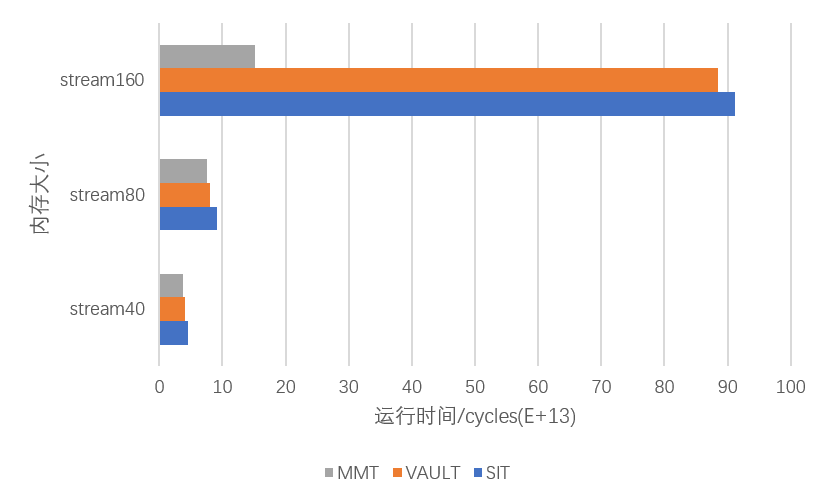
\includegraphics{eval-memorysize.png}
    \caption{\textbf{STREAM测试集使用内存大小与不同完整性保护方案下性能关系图}。}
   \label{fig:eval-memorysize}
\end{figure}
如图 ~\ref{fig:eval-memorysize}所示,我们比较程序使用不同的内存大小,对完整性检查的影响,在这里我们选取了STREAM测试集。STREAM是为了测试内存的性能的测试集,拥有较大的内存压力,频繁的读写内存能够快速耗尽SoC上能保护得安全内存得空间,同时产生频繁得swap操作。这里我们分别选取了SIT, VAULT, MMT对使用40M, 80M, 160M内存
得STREAM测试集做了分析。当程序使用的内存少于SoC上能够保护得内存时候,SIT,VAULT,MMT之间得差距并不是很明显。SIT会比MMT慢20\%左右,和VAULT相比,MMT采用了三级counter得设计,与VAULT相相比略有性能提升。因为40M和80M得内存较少,没有充分发挥三级counter得优势,当进一步扩大内存得时候三级counter得优势会更加的明显。
当使用的程序使用的内存超过了128M得时候。SIT和VAULT得性能开销急剧增加,因为STREAM会频繁循环的的访问内存,所以一旦超出了SoC上能够保护的内存时,就会频繁的发生swap操作,造成较大的性能开销。和SIT,VAULT相反,MMT采用了挂挂载的方式代替内存的swap,挂载操作的开销非常小(100~200 cycles)。所以当使用的内存扩大了一倍,
运行时间也线性的扩大了一倍,挂载操作并没有成为性能的瓶颈。而swap操作会带来7,8倍的性能开销,说明swap操作取代了完整性保护的检查,成为了主要的瓶颈。

\begin{figure}[hbt]
    \centering
    \setlength{\belowcaptionskip}{0pt}
    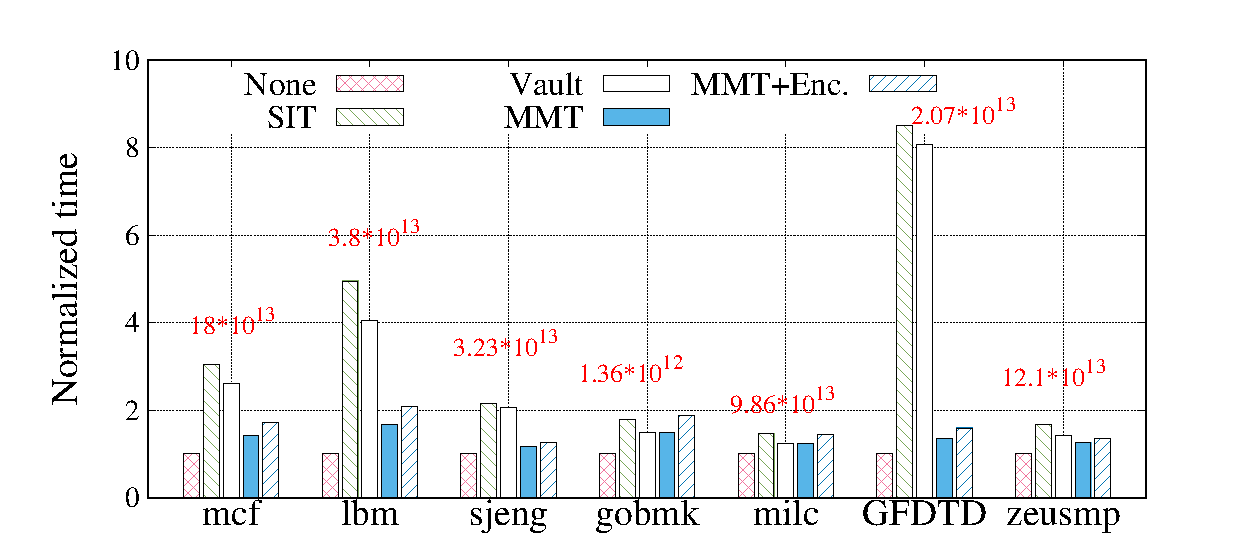
\includegraphics[scale=0.6]{fig/eval-integrity-bench.eps}
    \caption{\textbf{SPECCPU测试集在不同完整性保护方式下的性能}. \emph{None} 表示没有完整性保护下的理论性能。}
    %Compared with SGX and Vault, {\forest} can achieve the best performance in all the cases.
    \label{fig:eval-inter-bench}
\end{figure}
如图~\ref{fig:eval-inter-bench}所示,我们在SPECCPU上测试了SIT, VAULT, MMT, MMT+encrypt, 以及不做完整性检查原始的测试。其中\emph{gobmk},\emph{milc}两个测试集使用的内存小于128M,不会产生swap的开销,剩下的测试程序使用的内存从[180M:1200M]不等。从测试结果中我们可以发现,MMT的性能均优于SIT和VAULT,
在mcf的测试中,SIT和VAULT相较于没有完整性保护的程序分别会有2.05x和1.6x的开销,而MMT只有0.4x的开销,这部分的开销主要是完整性检查的开销,而挂载的开销小于1\%(挂载的操作只需要100~200的开销),在其他的测试中例如GemsFDTD,SIT和VAULT相较于不做完整性检查的程序来说有高达7.5x和7.06x倍的性能开销,而MMT只会
有0.35x的性能的开销。在这种极限的场景下,MMT相较于没有完整性保护的原程序来说只有0.35x的开销,Mount操作大幅减少了原有的swap的开销,并且在绝大多数的场景下,Mount的开销可以忽略不记(<1\%)。当使用内存小于SoC上可以保护的内存时候,MMT和Vault相比性能相近(这里为了是SoC上保护的内存相同,我们减少了MMT树的个数,因此三级counter的优势没有很好的体现)。
根据上面的测试我们可以得出,不论在内存使用超过SoC能保护的内存大小,还是小于SoC保护的内存时候,MMT都具有最好得性能,特别是当使用得内存超过SoC保护得内存大小得时候,挂载操作将极大得缓减原本swap页所带来的开销,又因为在运行时,可以通过Mount Table中读取子树的根节点来保证运行时候对完整性树检查的层数不变,从而保证SoC上内存足够的情况下,也不会带来额外的开销。

\section{性能评估}
通过以上的测试结果我们发现,对于传统的页交换操作,当使用的内存操作了SoC上能够保护内存大小的时候,会带了及其严重的性能开销,在极端的场景下,能够达到近十倍的性能下降。如此大的性能开销是完整性保护系统不可以接受,这也是为什么已有sgx的应用会指明使用的内存应该小于128M(EnclaveDB)。而对于挂载(Mount)操作,在最严重的场景下,其开销不会超过1\%,因为Mount带来的
开销相较于完整性检查可以忽略不计。因为Mount的存在,我们不需要在SoC中保护所有的内存,而只需要保护当前活跃的数据。因为内存访问的局域性,程序某一个时间段内存访问的内存将远小于它总共使用的内存,因此将大多数的子树放在内存是可行的,同时也是的MMT能够保护的内存大小达到TB级别。MMT不仅能够将保护的内存范围扩大几个数量级,同时也能够实现可扩展的内存分配,离散的内存保护。
在传统得完整性保护树中,只能够保护一块连续的固定的内存空间,并不能够动态的扩展该内存大小,同时也无法保护离散的内存区域。这些缺陷都限制了内存完整保护的可扩展性,并不是适应于云场景的环境。MMT的提出使得云场景中内存完整性保护成为了可能,结合内存隔离与加密技术,能够实现内存强安全保障。

MMT的性能也会受到以下几个因素的影响。一、虽然MMT支持离散内存的完整保护,但是在个别离散的场景中,会带来较大的性能开销。例如在每一颗一个子树中,只保护一页大小的内存完整,如果有一个程序恰好使用这些内存,那么每次的访问都有可能产生Mount与Unmount操作,从而带来较大的性能开销。然后在真实的场景中,这样的内存访问模式是很难产生的,因为程序具有一定的局域性,并且操作
系统也能够辅助,将程序使用的内存都分配在一起,缓解内存过于离散造成的频繁的挂载与卸载操作。二、在多核多cpu的场景下,为了保证每一个核至少有一个子树能够使用,Mount Table中保存的子树的个数应该至少超过cpu中的核数,这样才能够保证不会出现不同的核相互卸载其他核正在使用的子树。我们认为,Mount Table的大小应该是和核数成正相关,在多核的场景下,SoC上也会有更多的空间,
用于存储必要的信息。三、Mount操作在极端的场景中可能比页交换的次数还要多,例如程序对内存的访问刚好只访问子树中的个别几个页,从而导致频繁的子树切换。而对于页交换策略,因为只需要访问子树中的个别几个页,一段时间内使用的内存并不多,因此不会产生频繁的页替换。虽然页替换的次数可能小于挂载的次数,但是由于页交换需要40k cycles而Mount只需要100\sim200 cycles。所以Mount所花
的时间还是远小于页交换的时间。又因为一棵子树的大小为4M远大于页4K的大小,因此在一般的场景下,Mount操作的次数将远小于页交换的次数,结合Mount本身较少的操作时间,使得Mount所带来的开销几乎可以忽略不记。

